\documentclass[openany]{book}
\usepackage{graphicx} % Required for inserting images
\usepackage{amsmath}
\usepackage{enumerate}
\usepackage{enumitem}
\usepackage{epigraph}
\usepackage{lipsum}
% \usepackage{titlepages}
\usepackage{tikz}
\usepackage[a4paper, total={6in, 8in}]{geometry}

\usepackage{lipsum}
\usepackage[Glenn]{fncychap}
\renewcommand{\chaptername}{UNIT}
\ChNameUpperCase
\ChNumVar{\fontsize{40}{42}\usefont{OT1}{ptm}{m}{n}\selectfont}
\ChTitleVar{\Large\sc}

\title{Sociology 141 - Social Movements \& Political Action}
\author{Alejandro Sanchez Ocegueda}
\date{Last updated: \today}

\newcommand{\st}{$^{\text{st}}$}
\newcommand{\nd}{$^{\text{nd}}$}
\newcommand{\rd}{$^{\text{rd}}$}
\renewcommand{\th}{$^{\text{th}}$}

\renewcommand\epigraphflush{flushright}
\renewcommand\epigraphsize{\normalsize}
\setlength\epigraphwidth{0.7\textwidth}

\definecolor{titlepagecolor}{cmyk}{1,.60,0,.40}

\DeclareFixedFont{\titlefont}{T1}{ppl}{b}{it}{0.5in}

\makeatletter                       
\def\printauthor{%                  
    {\large \@author}}              
\makeatother
\author{%
    Sociology 141 - Spring 2025 \\
    Alejandro Sanchez Ocegueda \\
    % Updated \today \\
    \texttt{alexso@berkeley.edu}\vspace{20pt}
    % Department name \\
    }

% The following code is borrowed from: https://tex.stackexchange.com/a/86310/10898

\newcommand\titlepagedecoration{%
\begin{tikzpicture}[remember picture,overlay,shorten >= -10pt]

\coordinate (aux1) at ([yshift=-15pt]current page.north east);
\coordinate (aux2) at ([yshift=-410pt]current page.north east);
\coordinate (aux3) at ([xshift=-4.5cm]current page.north east);
\coordinate (aux4) at ([yshift=-150pt]current page.north east);

\begin{scope}[titlepagecolor!40,line width=12pt,rounded corners=12pt]
\draw
  (aux1) -- coordinate (a)
  ++(225:5) --
  ++(-45:5.1) coordinate (b);
\draw[shorten <= -10pt]
  (aux3) --
  (a) --
  (aux1);
\draw[opacity=0.6,titlepagecolor,shorten <= -10pt]
  (b) --
  ++(225:2.2) --
  ++(-45:2.2);
\end{scope}
\draw[titlepagecolor,line width=8pt,rounded corners=8pt,shorten <= -10pt]
  (aux4) --
  ++(225:0.8) --
  ++(-45:0.8);
\begin{scope}[titlepagecolor!70,line width=6pt,rounded corners=8pt]
\draw[shorten <= -10pt]
  (aux2) --
  ++(225:3) coordinate[pos=0.45] (c) --
  ++(-45:3.1);
\draw
  (aux2) --
  (c) --
  ++(135:2.5) --
  ++(45:2.5) --
  ++(-45:2.5) coordinate[pos=0.3] (d);   
\draw 
  (d) -- +(45:1);
\end{scope}
\end{tikzpicture}%
}

\begin{document}
\begin{titlepage}
\noindent
\titlefont Social Movements \par
\epigraph{Pure mathematics is on the whole distinctly more useful than applied. For what is useful above all is technique, and mathematical technique is taught mainly through pure mathematics.}%
{\textit{London 1941}\\ \textsc{G. H. Hardy}}
\null\vfill
\vspace*{1cm}
\noindent
\hfill
\begin{minipage}{0.35\linewidth}
    \begin{flushright}
        \printauthor
    \end{flushright}
\end{minipage}
%
\begin{minipage}{0.02\linewidth}
    \rule{1pt}{125pt}
\end{minipage}
\titlepagedecoration
\end{titlepage}

\tableofcontents

\chapter{Social Movements \& Sociology}
This unit introduces the theoretical foundation for the class, drawn from Piven \& Cloward's seminal work \textit{Poor People's Movements: Why They Suceed, How They Fail}.
The principal social movement studied in this unit is the Movement of the Unemployed, which took place during the Great Depression, largely due to a period of rapid economic and social change.
\vspace{5mm}

% Date: January 21st

\counterwithout{section}{chapter}
\noindent \textbf{Lecture 1 --- January 21\st}

\section{Approaches to Social Movements}
In this first section, we first give a brief overview of the different approaches to studying social movements and political action.


\subsection{The Pluralist Approach}
% TODO
The argument of the pluralist was that the US was good because the system included a plurality of interests (hence the name).
The idea was that even if there were imbalances and inequalities, the political power was widely distributed between competing groups;
that is, no one group completely controls the system.


\subsection{The Classical Approach}

The classical approach refers to the way scholars and sociologists studied social movements before the 1970s.

Fun fact: the course is titled \textit{Social Movements \& Political Action}.
In the classical approach.

Aside: Political Action.
Before, the study of social movements was relegated to social psychology, mostly because it was viewed as an irrational action.
It was categorized as a form of ``deviance.''
They were viewed as ``pathological'' or ``irrational''.

% \section{Political Sociology}

Political Science and Political Sociology studied Institutional Politics, whereas Social Psychology studied Insurgent Politics

\textbf{Institutional Politics:} Politicis within formal institutional channels.
For instance, electoral processes.
During the classical times, only institutional politics were viewed as ``real'' politics. 
Other forms of politics (often known as insurgent politics) were viewed as ``not real'' politics.

\noindent \textbf{Insurgent Politics:} Collective behavior (?)

Pluralist approach $\Rightarrow$ Classical approach

The classical approach is based on the pluralist approach to politics.


The underlying assumption is that the competition between the different political groups would balance out the disparity among them.
This, in theory, ensured that the political system was
\begin{enumerate}
    \item \textbf{Open:} no group monopolizes power to block other groups.
    \item \textbf{Responsive:} the need for coalitions necessitates responding to the demands of other groups.
\end{enumerate}

This was the dominant theory during the 1960s.

C Wright Mills refers to this as ``Elite Theory.''

\subsection{The Elite Theory Approach}
This is a new approach first proposed by C. Wright Mills, and it centers around the concept of the ``elite.''

\noindent \textbf{Elite:} those who hold power in a society.
The idea transitioned from the Elite Theory to the Resource Mobilization approach.

The postulates of Elite Theory are as follows:
\begin{enumerate}
    \item The system is controlled by the elite
    \item Most groups are politically excluded
\end{enumerate}

\subsection{The Resource Mobilization Approach}
This new approach is based on the Elite Theory approach to politics. 

\subsection{Why care about all these approaches?}
Today, all of this falls under the ``Political Action'' umbrella term.
Furthermore, the classical approach has been completely rejected.
But why is it worth our time?
In part, it is important to know about these things because understanding these old approaches gives you a sense of what newer scholars are arguing against.
Most importantly, it is important to understand how social movements were often cast to the wayside and treated as irrational and deviant.
These ideas and assumptions, antiquated and refuted as they are, continue to shape the way people think and approach social movements to this very day.


\section{Social Movements}
There are several questions we will address throughout this course

\begin{enumerate}
    \item Emergence: under what conditions do mass social movements to emerge?
    How can we learn to recognize those conditions so that we can fully exploit them when they show up?
    \item Objectives:
    What have social movements sought to achieve?
    \item Strategies/Tactics: What different kinds of tactics have been used to attain those objectives? 
    Which strategies and tactics have been effective?
    What factors influence the efficacy?
    \item Organization:
    How have different movements organized themselves?
    What different forms of organization have they adopted?
    \item Challenges:
    What kinds of challenges have different movements faced?
    What different state oppression have movements been challenged with?
    How have different movements responded or adapted to those challenges?
    \item Impact:
    How can we fully assess the impacts of movements?
    What have been their intended impacts?
    What have been the unintended impacts or reverberations of social movements?
\end{enumerate}


% \counterwithout{section}{chapter}

\vspace{3mm}
\noindent \textbf{Lecture 2 --- January 23\rd}

\section{The Structuring of Protest}
At the heart of sociology, there is an ongoing debate between the importance of agency and structure.
Agency is defined to be the capacity of human beings to act independently.
Structuralism is a branch of sociological belief that emphasizes that agency is shaped and constrained by the structures of society.
One can think of this debate as a continuum, where all sociologists lay in some point, giving more or less important to agency and structure.

\begin{center}
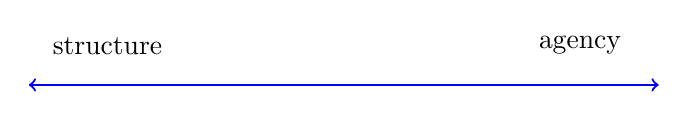
\begin{tikzpicture}
    \draw[thick, <->, blue] (0,0)  -- (8, 0);
    \draw (1, 0.5) node{structure};
    \draw (7, 0.5) node{agency};
    \draw[.] (5,0);
\end{tikzpicture}
\end{center}

Q: Is agency required for structure to arise?

Piven and Cloward make a structuralist argument regarding social movements.
More specifically, they argue that the structure of society influences when movements can arise, what shape the movements will take, and how effective they will be.

\begin{center}
\textit{``In seeking to do what wasn't possible, we failed to do what was... (p. TODO)''}
\end{center}

Notably, Piven \& Cloward offer their own ideas of what a social movement is.
In other words, what should count as a social movement (pp. 3-4).
The two main criteria that they propose are that there should be (a) a transformation of consciousness, and (b) a transformation of behavior.

\subsection{Transformation of Consciousness}
We summarize the criteria that Piven \& Cloward give for a transformation of consciousness below:
\begin{enumerate}
    \item \textit{The system loses legitimacy:}
    In other words, people view the structure of society as unjust and wrong.
    This should not be surprising.
    In fact, most people, at most points in time, believe that society is unjust and wrong (at least to some extent).
    However, this is still an important and necessary condition for a social movement to arise (at least according to Piven \& Cloward).
    \item \textit{Alternatives seem possible:}
    Unlike most of the time, people think that there indeed does exist another way of living.
    \item \textit{Sense of efficacy:}
    Finally, the people come to believe that not only is the system wrong and that there exists a viable alternative, but that this alternative is indeed something that is attainable.
\end{enumerate}
There is a sort of implicit precedence between these three criteria.
Before people think that they can change their living situation to something better, they must have an idea of what the alternative is in mind, and before people conceive that alternative, it is necessary that they see something that is wrong and requires change within their current conditions.

\subsection{Transformation of Behavior}

\begin{enumerate}
    \item \textit{Masses of people become defiant:}
    By this, we mean that people begin to break the rules and norms established in society.
    These can be formal rules (such as the law), or cultural rules.
    Not all movements break the law, but all movements break some form of social norm.
    \item \textit{Defiance is acted out collectively:}
    It is not only necessary that rules and norms are broken by the people, but that people engaging in this disobedience also believe that they are acting as part of a larger group or movement.
\end{enumerate}
Succinctly, we can say 
\begin{center}
\textit{``A protest movement is collective defiance fueled by a transformation of consciousness.''}  
\end{center}


\section{Emergence of Protest Movements}
Now that we have discussed \textit{what} social movements are, a natural question to ask is \textit{when} social movements \textbf{emerge}.
Piven \& Cloward give a characterization for the conditions necessary to spark a social movement.

\begin{enumerate}
    \item \textit{Massive social or economic changes:}
    There must be a rapid and drastic change in the living conditions of a large group of people.
    This can be a massive migration, industrialization, depression, or any other number of such large-scale events.
    \item \textit{Institutional breakdown:}
    The aforementioned massive social/economic changes begin to strain the institutions.
    For example, an economic force like a depression can put a lot of strain on a number of institutions.
    This, importantly, disrupts the routines of people's daily lives.
    \item \textit{Transformation of consciousness:} 
    These two conditions put together, cause a profound \textbf{social dislocation}.
    Informally, people's lives are thrown out of whack.
    This is often sufficient to cause a transformation of consciousness, of the kind we had defined and talked about at length previously.
    \item \textit{Division \& competition among elites:}
    The vested interest of the ruling class is in preserving the status quo.
    Mostly, they are unified in their interest in maintaining the status quo.
    Nonetheless, periods of massive economic change and social upheaval can create fissures among the elite class.
    This can cause dissonance and delegitimize their authority.

\end{enumerate}
Once again, Piven \& Cloward provide us with a fancy quote to characterize these criteria:
\begin{center}
\textit{``The social arrangements that are ordinarily perceived as just and immutable must come to be perceived as unjust and mutable (p. TODO).''}
\end{center}

\newpage
\noindent \textbf{Lecture 3 --- January 28\th}

% The main argument of Piven \& Cloward's work is that possibilities for protest movements are \textbf{structurally shaped and constrained}.
% The defining feature of a movement is \textbf{collective defiance}.

% Institutions of society begin to strain and break down.

\section{Methods of Protest Movements}
How can we understand the different methods and tactics employed by different movements?
Why do some people block freeways, while others burn down police stations, and others peacefully take to the streets to march?
Moreover, why don't people try to work \textit{with} the system instead of \textit{against} it?

\subsection{Strategy: Electoral Politics}
It turns out that the very first step to a protest or social movements is actually a change in electoral politics.
In other words, every social movement\footnote{At the very least, every social movement that we cover in Sociology 141.} has been preceded by a notable change in voting patterns.
This indicates that people \textit{do} indeed turn to the electoral system before breaking out of it.
However, Piven \& Cloward also observe that, after enough empty promises and unmet needs, people can (and will) pursue their goals through non-electoral means.

\subsection{Factors}
What determines the different methods that people use?

\begin{enumerate}
    \item 
    \textit{Concrete experiences of daily life:}
    These shape grievances and determine the targets of the protest.
    For instance, people will not rebel against capitalism, they will rebel against their employer who treats them unfairly.
    Similarly, the unemployed will not protest against social policy, but rather against the relief bureaucracy that directly affects their daily lives.
    \item 
    \textit{Structuring of collectivities:} 
    This refers to how people are aggregated.
    For instance, factory workers are aggregated in a factory, where they can share their experiences and collude.
    On the other hand, 
    \item 
    \textit{Disruptive impact:}
    This is determined by structural positioning.
    % TODO: rewrite this bc it's wordy and hard to read
    Defiance is only effective insofar as it disrupts the institutions against which they are.
    Stated differently, there must be some threat of interrupting the status quo on part of the movement.
    Disruptive impact can come about through withholding labor, consumption, by rioting, and many, many others.
\end{enumerate}
In the sections that follow, we will spend some time working on specific strategies .

\subsection{Strategy: Disruption}
We define \textbf{disruption} as collective defiance (or withholding of cooperation) to cause an interruption to the regular flow of institutional operations.
As long as the institution does not provide change, social movements will resort to disrupt the system until some change comes about.
At its core, every social movement has some aspect of disruption.
that has brought about change has done so through \textit{some} form of disruption.
Disruption forces, at the very least, that the system pays attention, and it often also forces the system to change.

One form of disruption is the \textbf{riot}.
Riots can be conceived of as a \textit{disruption of public order}.
They are often shamed by the public view and dismissed as   ``irrational.''
But, as it turns out, riots are in fact highly rational actions taken by people who are so oppressed by the system that they cause disruption in the one place that they have power:
maintaining the public order.

A common criticism about movements is that they are ``too disruptive.''
This point of view misses the entire \textit{point} of social movements.
To put it differently, the people complaining about the Palestine protests at graduation have a serious fundamental misunderstanding of what a protest is even supposed to be.
% Riots disrupt public order.
% A rebellion is a more general term that describes the movement itself.


\begin{center}
    Collective defiance $\Rightarrow$ Institutional Disruption $\Rightarrow$ Political Reverberations (concessions).
\end{center}
\vspace{3mm}
\noindent \textbf{Lecture 4 --- January 30\th}

\subsubsection{On Striking}
A strike is a tactic where people withhold labor.
Typically, strikes happen at the level of one company.
There are also industry-wide strike, in which workers of a given industry withhold labor.
A general strike is an extreme case of this.
In a general strike, \textit{all} workers within a general area go on strike.
We

\section{The Movement of the Unemployed}
We now want to pay attention to how the Movement of the Unemployed illustrates Piven \& Cloward's theory of social movements.

\subsection{Emergence}
There were several notable components of P\&C's theory that are visible in the Movement of the Unemployed.
We describe them below.

\subsubsection{Massive social and economic changes}
This one is quite obvious.
The Great Depression came with drastic changes to the living conditions of everyone.
Many people became poor.


\subsubsection{Institutional Breakdown}
Regarding the institution of the family, the number of the divorces skyrocketed.
There was a massive increase in homelessness, indicating the breakdown of the institution of the home.
Malnutrition and disease rates.
Suicide rates also went up.

\subsubsection{Transformation of Consciousness}
People began to recognize the failures came at a systemic level.

Part of the reason why this was so crucial in the United States was because of the stigma and shame that poverty entailed.
Economic failure was deemed as a matter of personal failure.
However, the radical shift was from individual shame to collective indignation.

\subsubsection{Division \& competition among elites}
The very first division starts to happen between political officials at the local and federal level.

\subsubsection{Parallels to the Pandemic}
There are many parallels to the Great Depression and contemporary times.
These were unprecedented times.
Several industries shut down, people were being evicted, children could not go to school, etc.

\subsection{Objectives}
The main objective of the movement was to elicit a reaction from the government.
Specifically, they wanted to force concessions from the government, mainly relief.

\subsection{Strategies and tactics}
The main \textbf{strategy} of the Movement of the Unemployed was that of disrupting social order.
To incite disruption, they had several tactics.
These included but were not limited to: looting, rent riots (eviction defenses), and mass protests.
Another cool tactic was to reinstall water, gas, and electricity services after it was cut off by companies like PG\&E.
Relief insurgency (occupation) was done to try to force the hand of the people in power.

\noindent \textbf{Strategy:} Plans for achieving some objective of a social movement. 

\noindent \textbf{Tactic:} Methods (forms of action) through which the strategies are enacted.




\vspace{3mm}
\noindent \textbf{Lecture 5 --- February 6\th}

Class was sadly canceled due to the passing of Professor Michael Burawoy.

\vspace{3mm}
\noindent \textbf{Lecture 6 --- February 4\th}

\section{The Real Lesson from Baltimore}
This reading makes the overarching claim that ``riots work.''
It focuses on instances of police brutality, namely the killings of Freddie Gray, Michael Brown, and Oscar Grant.

\begin{center}
    \textit{Every concession is at the same time a containment strategy.}
\end{center}

\subsection{Organization}
There were Unemployed Councils in virtually every city, which were small, local organizations that would incite people to protest.

Later, there was the rise of the Workers Alliance of America, which Piven \& Cloward describe as a ``mass membership organization.''
There was a prevalent belief that there was a need to create these sorts of organizations, as they would enable the coordination of members, resources, and such that they could create a large voting block.
It is a belief that this kind of mass

Piven \& Cloward argue that these mass membership organizations were built off the success of disruption, and their very existence would undermine that same power of disruption.
One way this would happen was because the leadership of these organizations would get distracted by institutional politics, and focus more on building up the organization building than in attaining the goals of the movement.

Dangers of concessions:
Co-optation, fragmentation of the movement, and more.
Furthermore, the concessions were by no means equally distributed once they were received.
\vspace{3mm}
% \noindent \textbf{Lecture 6 --- February 6\th}
\setcounter{section}{0}




\section{Emergence of Movement (Insurgency)}
This is a classical political theory book by Doug McAdam.
In this text, McAdam argues that there are some conditions that must be met before the rise of a movement:
\begin{enumerate}
    \item Structure of Political Opportunity
    \item Indigenous Organizational Strength
    \item Cognitive Liberation
\end{enumerate}

\subsection{Structure of Political Opportunity}
The alignment of groups within the larger political environment.
Another way to put it is as  ``a shift in the balance of power relations'' at any given moment.
There are moments when the balance of power relations is shifted, creating an open for insurgency.
Insurgents have leverage or power that they didn't have before.
Alternatively, the ability of the elites to repress the movement freely, the ``cost of repression,'' if you will, is diminished.

\subsection{Indigenous Organizational Strength}
The concept of \textit{Indigenous Organizational Strength} can be conceived of as the organizational readiness to exploit political opportunity.


\subsection{Cognitive Liberation}
The collective liberation of the movement...
This is almost the same concept as Piven and Cloward's ``transformation of consciousness.''

\section{Development/Decline of Movement}

\subsection{Structure of Political Opportunity}
The balance of power relations is dynamic.
\begin{enumerate}
    \item Structure of Political Opportunity
    \item Organizational Strength
    \item Collective Attribution
    \item Social Control Responses
\end{enumerate}

\subsection{Organizational Strength}
In the long run, indigenous organizations are not enough to sustain a movement.
In fact, he argues (in opposition to P\&C) that formal organizations are necessary for centralized coordination.
However, these centralized formal institutions come with dangers:
\begin{itemize}
    \item Oligarchization
    \item Co-optation
    \item Disconnection from indigenous base
\end{itemize}


Civil rights organizations
\begin{itemize}
    \item NAACP - National Association for the Advancement of Colored People
    \item CORE - Congress of Racial Equality
    \item SCLC - Southern Christian leadership Conference
    \item SNCC - Student Non-Violent Coordinating Committee
\end{itemize}

\vspace{3mm}
\noindent \textbf{Lecture 7 --- February 11\th}

\subsection{Collective Attribution}
This is basically the same as Piven \& Cloward's concept of ``cognitive liberation.''

\subsection{Social Control Responses}
We are taught that in the traditional liberal view, the government is an ally working in favor of the goals of the movement.
McAdam challenges this view, and instead says that if anything, the government is attempting to maintain a neutral position and avoid antagonizing either side too much.

% \section{Nonviolence}
% This is a concept that is perhaps antithetical to the point of social movements.

\section{Tactical Innovation}
\subsubsection{Black Insurgency (1955-1970)}

\begin{enumerate}
    \item \textbf{Structure of Political Opportunity:}
    One big evolution along this axis is that Black insurgents found themselves in a position where they had more leverage, while the cost of repression also became higher.
    \begin{enumerate}
        \item $\uparrow$ Black electoral power.
        \item Collapse of southern cotton economy $\rightarrow$ urban migration.
        \item $\uparrow$ Significance of Third World\footnote{In Cold War lingo, Third World countries were countries that were not aligned with NATO or the Warsaw Pact.} to US foreign policy (Cold War)
        
    \end{enumerate}
    \item \textbf{Indigenous Organizational Strength:}
    \begin{enumerate}
        \item Black Churches
        \item Black Colleges
        \item Southern Wing of the NAACP
    \end{enumerate}
    \item \textbf{Cognitive Liberation:}
    This is not explicitly mentioned by McAdam in the reading.
    However, McAdam does mention that the insurgents must feel that ``the time is right.''
    \item \textbf{Social Control Responses:}
    These shape the movement's ability to either develop or decline.
\end{enumerate}

\section{Significance of Disruptive Tactics}

Challengers lack institutional power $\Rightarrow$ Must resort to non-institutional tactics that force a response.

\begin{enumerate}
    \item Bus boycotts
    \item Sit-ins
    \item Freedom rides
    \item Community campaigns
    \item Riots
\end{enumerate}

\section{Tactical Interaction}

Tactical Innovation: the creativity of insurgents in devising new tactical forms.

Tactical adaptation: the ability of opponents to neutralize these moves on 

% TODO: draw circle of tactical innovation and tactical adaptation


\vspace{3mm}
\noindent \textbf{Lecture 8 --- February 13\th}


\section{Civil Rights Movement}

\begin{itemize}
    \item[[ 1954]] Brown vs Board of Education, Muder of Emmett Till
    
    \item[[ 1955]] Montgomery Bus Boycott

   \item[[ 1960]] Grensboro Sit-ins
   \item [[ 1961]] Freedom Rides
\end{itemize}


\subsection{Emmett Till (1954)}
A 14-year-old black boy who was falsely accused of flirting with a 21-year-old white woman.
He was beaten to death and then his body was thrown in to a river.

\subsection{Boycott}
A boycott is a tactic in which individuals abstain from consumption.
It is similar to a strike, in which workers withhold labor.
Here, consumers withhold consumption.
The idea is to cause economic disruption.

\subsection{Sit-in}
A sit-in is the organized occupation of space and refusal to leave until demands are met.

Form of Occupation -- physically taking over space in a manner that lays claim to and prefigures new uses for it.

\subsection{Freedom Rides}
Sending biracial groups (freedom riders) to ride buses throughout the south.
They were going around challenging segregation in those facilities.
The purpose was to place pressure on the government to force them to act on the ruling.
Their aim was economic disruption through the segregationist violence.



\subsubsection{Adaptations}
There were several adaptations that resulted.
On the legal end, the governments would give citations/arrests to boycotters.
On the extralegal end, there was a lot of violence (beatings, bombings, and more).


In 1960, JFK defeats Richard Nixon by less than $\frac{1}{3}$ of the popular vote:
$49.7\%$ vs $49.5\%$.

\section{Strategy of Direct Action}
Instead of acting through elected officials, acting outside of formal institutional politics in order to achieve the group's objectives.


\section{Strategy of Civil Disobedience}
A strategy of intentionally breaking the law.


% \chapter{The Power of Disruption: The Movement of the Unemployed}


% \newpage
% \chapter{Strategic \& Tactical Dynamics: The Civil Rights Movement}

% \chapter{Unintended Impacts: Countermovements \& Electoral Reverberations}

% \chapter{``Free Speech'': UC Berkeley from the FSM to the Palestine Solidarity Movement}

% \chapter{``Black Power'' and its Progenies: The Black Panther Party \& the New Left}

% \chapter{The Dynamics of Repression}

% \chapter{The Stonewall Riots \& the Gay and Trans Liberation Movements}

% \chapter{Occupy \& the ``Violence'' of Resistance}

% \chapter{The Dialectic of Repression \& Resistance: ``Black Power'' to ``Black Lives Matter''}

% \chapter{Indigenous Resistance: From ``Red Power'' to Standing Rock}

% \chapter{The Movement for Black Lives}




\end{document}